\section{System Architecture}
\label{architecture}

In this section, we discuss SYSTEM, a system for avoiding a specified country when accessing a webpage.

\subsection{Threat Model}
\label{threat}
This system is targeting an attacker who is at the nation-state level, and practices wiretapping on Internet traffic within the nation-state.  This type of attacker can appear on either the forward or reverse path, as shown in Figure~\ref{fig:attacker}. An attacker can also conduct surveillance on parts of webpages by being on the path from the client to some source that is requested by an initial page load; for example, a client accesses foo.com, and foo.com uses a Javascript file from bar.com, but bar.com is located in a different location.  An attacker can see the traffic between the client and bar.com, but not the client and foo.com.  This is depicted in Figure~\ref{fig:domains_attacker}.

\begin{figure}
\begin{minipage}[c][11cm][t]{.5\textwidth}
  \centering
  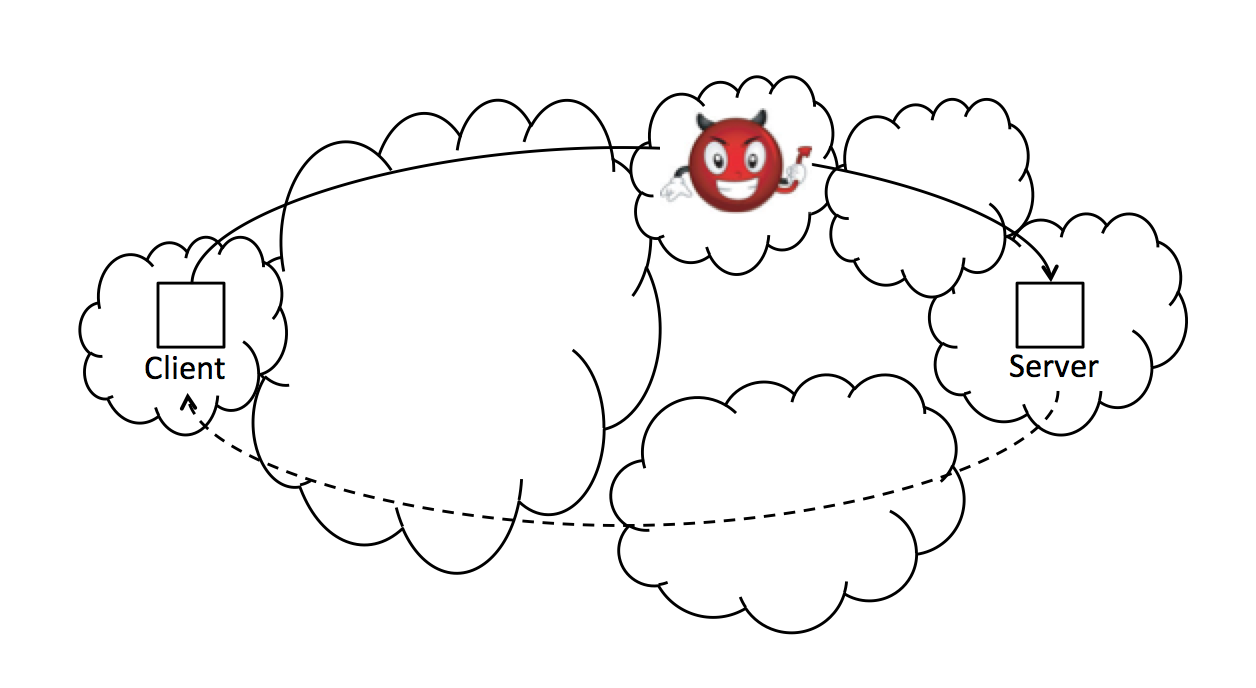
\includegraphics[width=.99\textwidth]{forward_evil}
  \subcaption{An attacker on the forward path.}
  \label{fig:forward_attack}\par\vfill
  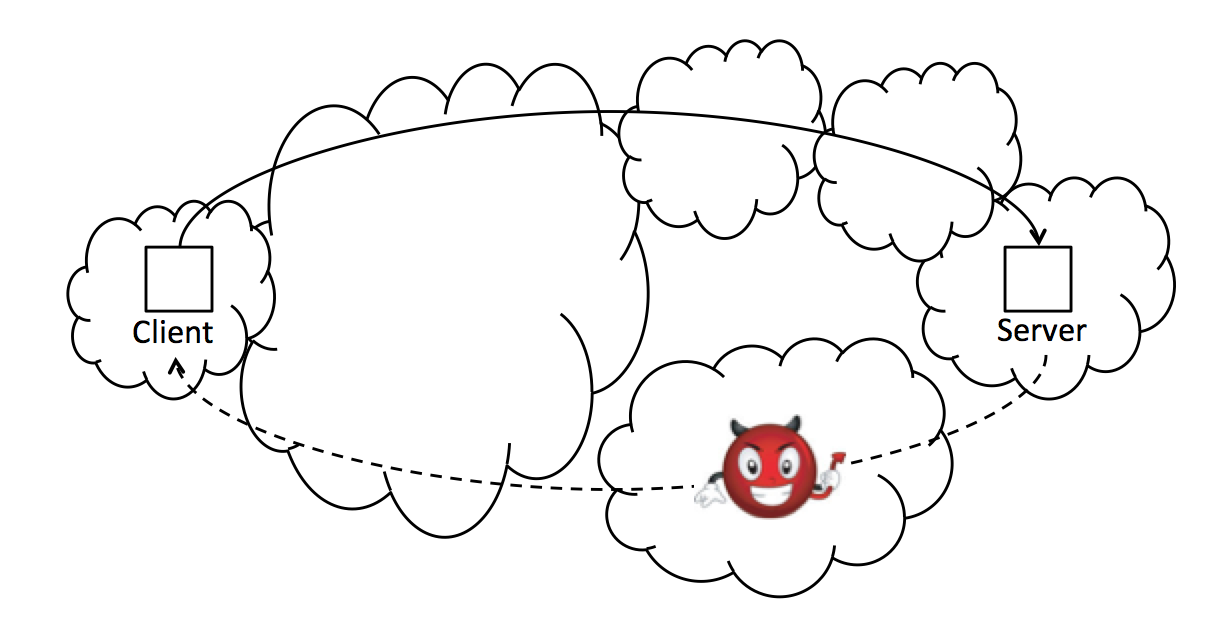
\includegraphics[width=.99\textwidth]{reverse_evil}
  \subcaption{An attacker on the reverse path.}
  \label{fig:reverse_attack}
\end{minipage}
\caption{An attacker can be on the forward or reverse path.}
\label{fig:attacker}
\end{figure}

\begin{figure}
\centering
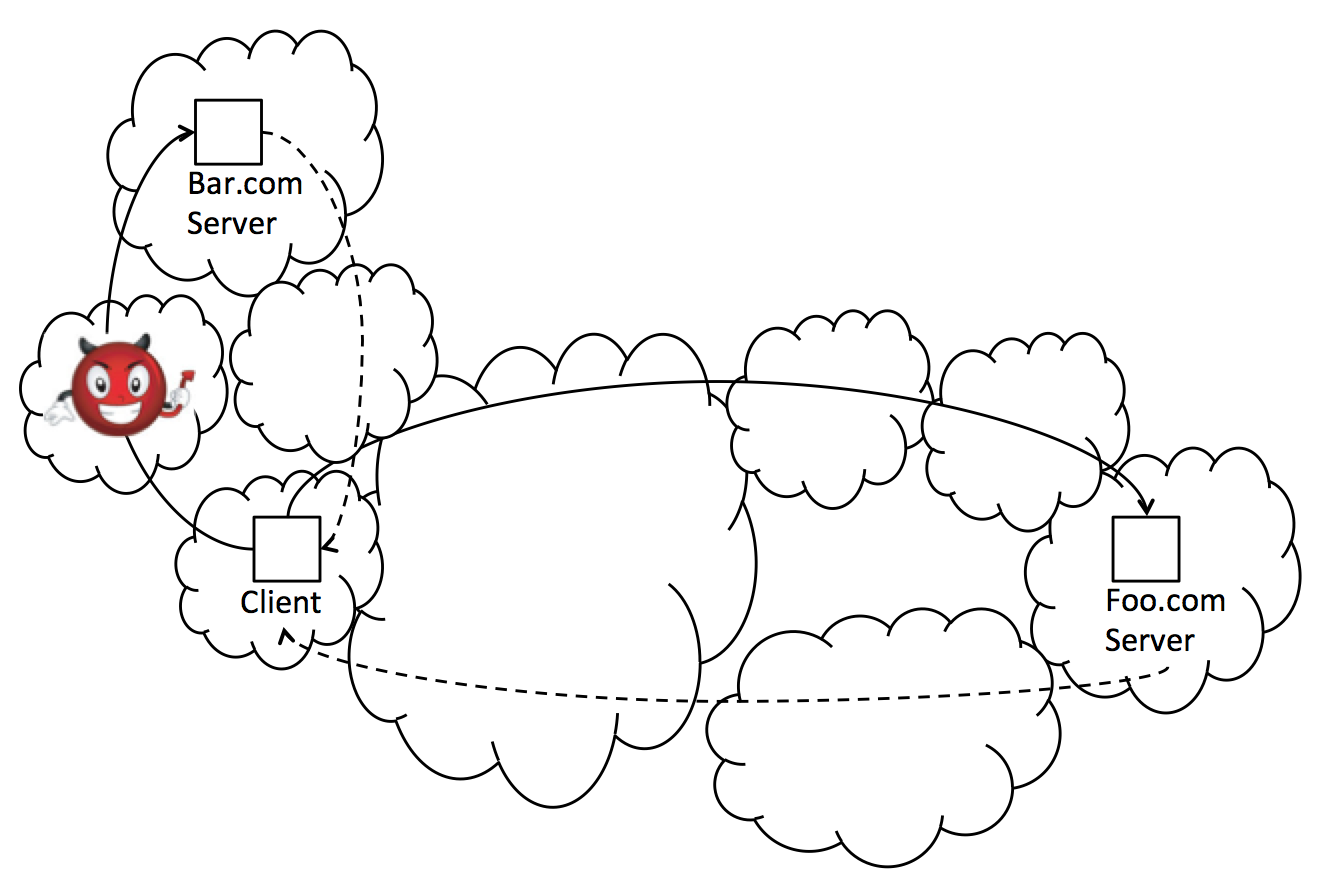
\includegraphics[width=.5\textwidth]{subsequent_request_attacker}
\caption{An example attacker on the path from the client to a third party domain's server (bar.com), which was fetched due to an initial request for foo.com.}
\label{fig:domains_attacker}
\end{figure}

\subsection{Design Goals}

With the attacker described in Section~\ref{threat} in mind, SYSTEM has three goals: singular country avoidance, avoiding colluding countries, and usability.  

{\bf Country Avoidance.}  The system should allow an Internet user, a client, to access web content without having her traffic travel through a country that she specifies, particularly countries that conduct surveillance.  The specified country should be avoided on both the forward and reverse paths, as they have been shown to be asymmetric, and thus a country may be on the reverse path, but not on the forward path~\cite{he2005routing}.  

{\bf Colluding Countries Avoidance.}  There have been agreements between countries to share surveillance data; this is analagous to colluding adversaries~\cite{fiveeyes}.  This system will allow clients to specify multiple countries to avoid, and the system will attempt to avoid all specified countries.  For the purposes of simplicity, the examples and descriptions in this paper will include only one country to avoid, but the system will be designed to handle multiple colluding countries.

{\bf Usability.} In order for the system to be used, it must be usable from both the client- and server-side.  All participants in the system must be required to do as little work as possible to use the system.  We envision the system growing, and our goals for the long-term would also be scalability and performance.

We assume that relays, clients, servers, and oracles are not malicious, and that no other attacks, such as Man-in-the-Middle, BGP prefix hijack, etc., are occuring.

\subsection{Architecture Overview}

Figure~\ref{fig:overview} shows the steps that occur when a client visits www.foo.com, using a standard browser. Both the oracle and the server maintain country-level path information, which is described in more detail in Section~\ref{maps}.

\begin{enumerate}
\item A client queries the oracle by supplying a domain and a country to avoid.  
\item The oracle searchs for a suitable relay, such that the specified country is not on the client to relay path, the relay to server path, and the relay to client path.  Once this relay is found, it responds to the client with the IP address of the relay.
\item The client sends the web request to the relay.
\item The relay forwards the request to the closest server that contains the domain.
\item The server determines if the server to relay path avoids the given country.  If so, then it sends the response to the relay. If not, then it will check if any of the geo-replicated servers have a path to the relay that does not include the given country; if there is such a path, then it uses it, otherwise, country avoidance is not possible for this request.
\item The relay forwards the response to the client.
\end{enumerate}

\begin{figure}
\centering
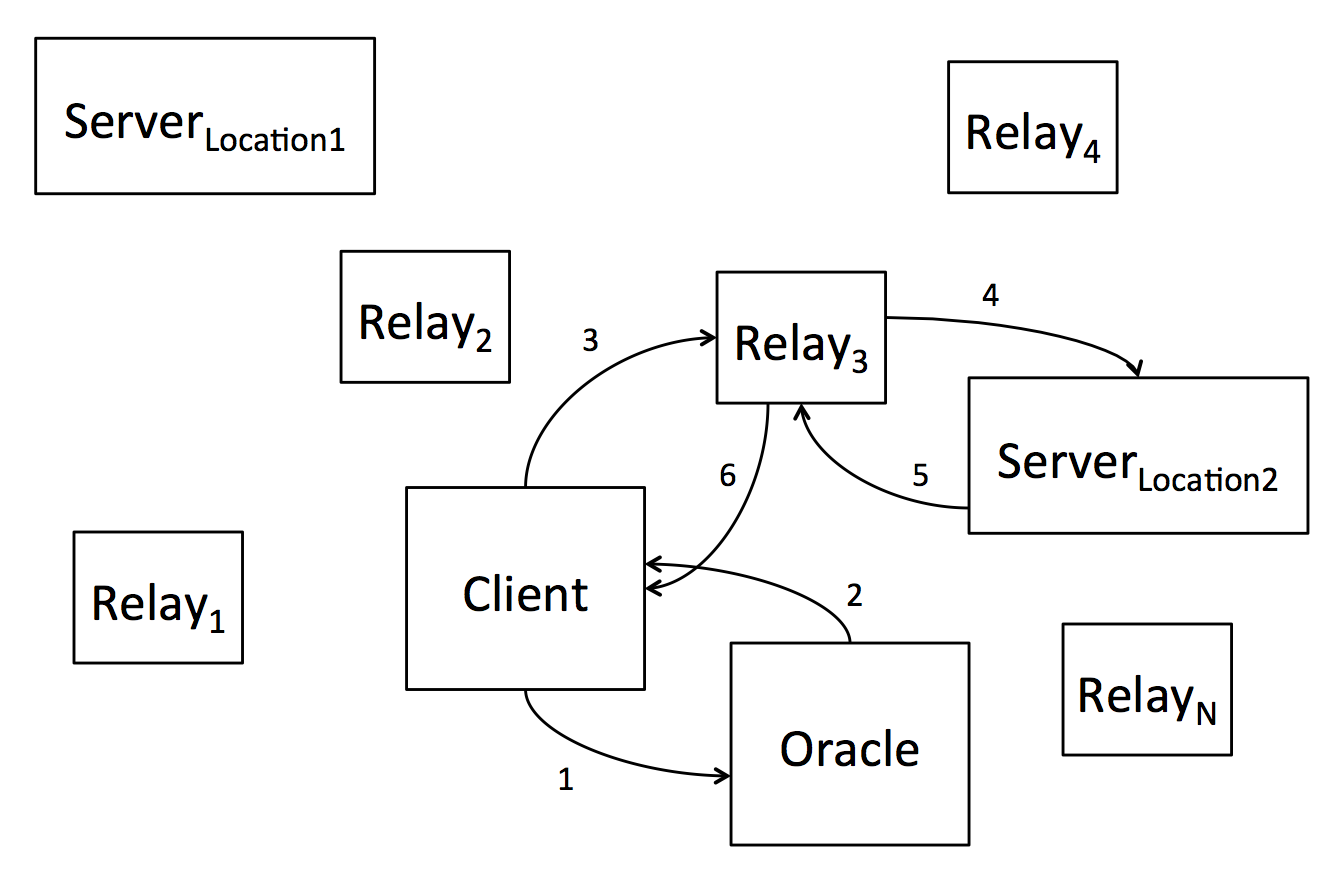
\includegraphics[width=.5\textwidth]{system_overview}
\caption{Using SYSTEM, the steps involved in requesting web content.}
\label{fig:overview}
\end{figure}

Based on this system design, we can see that there are more possible paths that an attacker can be on.  Figure~\ref{fig:advanced_threat} shows the possible places that a specified country (to be avoided) may be; these include the path from the client to the relay, the relay to the server, the server to the relay, and the relay to the client.  This increased attack space is because forward and reverse paths are asymmetric; research has shown that forward and reverse paths are asymmetric at the AS-level, but to our knowledge, no work has looked at the asymmetry of country-level paths~\cite{he2005routing}.  We found that the forward and reverse paths are asymmetric at the country level; we used RIPE Atlas probes to run traceroute measurements between pairs of probes.  Then we mapped the IP-level path to the country-level path.  Some country-level paths were symmetric, but we found others that were asymmetric; for example, a path from Brazil to Germany (189.112.0.1 to 185.13.208.1) has the country-level path Brazil $\rightarrow$ Venezuela $\rightarrow$ United States $\rightarrow$ Germany, whereas a path from Germany to Brazil (185.13.208.1 to 189.112.0.1) has the path Germany $\rightarrow$ Great Britain $\rightarrow$ United States $\rightarrow$ Brazil.  This shows that we cannot assume symmetric country-level paths. This is compounded by the secondary requests that are issued when the page is loaded on the client's browser.  

\subsubsection{Client} The client queries the oracle for a suitable relay and then uses that relay to access web content.  First, the client checks it's cache for the domain; if it is in the cache, then the client uses the relay IP address that is in associated with the domain in the cache.  It's important to note that the client's cache is refreshed twice as often as the oracle refreshes it's paths.  If the domain is not in the cache, then the client sends a query containing the domain and the country to avoid to the oracle.  The client will then recieve a response that is the IP address of a suitable relay for avoiding the specified country.  This (domain, relay IP address) pair will be added to the client's cache and the web request for the domain will be sent to the relay IP address.  Then the client waits for a response from the relay to display in the client's browser.  This process is repeated for each source that is requested during the web page load.  

\subsubsection{Oracle} The oracle contains information about the country-level path for the following source-destination pairs:

\begin{itemize}
\item Client to Relay
\item Relay to Server
\item Relay to Client
\end{itemize}

It contains these mappings for every client, every relay, and every popular server/CDN.  Once it receives a query from a client, it searchs the mappings for a relay such that the country to avoid is not on the client to relay path, relay to server path, and relay to client path.  Once a relay is found that satisfies these requirements, it sends the IP address of the relay to the client.  More information on the initialization, freshness, and maintenance of the mappings is discussed in Section~\ref{maps}.

\subsubsection{Relay} The relays act as proxies for clients so that it appears that a client is in a different geographic location; this allows the client to access the same web content on a different georeplicated server.  The proxy accepts requests from clients, locally resolves the domain, and forwards the request to the closest replicated server.  It then waits for a response from the server, and forwards it to the client.   

\subsubsection{Server} The server contains information about the country-level path for the server to relay path.  Once the server receives a web request, it checks it's mappings and if the country to avoid is not on the path from server to relay, then it sends the response to the relay.  If the country to avoid is on the path from server to relay, then it can check if any of it's georeplicated servers have a path to the relay that avoid the specified country.  If there is some server location that can avoid the specified country, then the response is sent from that server \annie{check the Internet Cache Protocol detail to see if this is feasible}.  Otherwise, the country is unavoidable, and response is sent through the specified country.

\subsection{Mapping Creation and Maintenance}
\label{maps}

Both the oracle and the servers must generate and maintain mappings of pairs of machines to the country-level paths.  The oracle must maintain the country-level paths from: all clients to all relays, all relays to all popular servers/CDNS, all relays to all clients.  The server must maintain the country-level paths from all of the georeplicated servers (for the domain) to all relays.  

The mappings for the oracle are initialized by using RIPE Atlas probes to conduct traceroute measurements from client subnets to all relays.  Traceroute measurements are also run from all relays to all popular servers/CDNs and to all client subnets.  Once these IP-level paths are calculated, the oracle uses a geolocation tool to map the IP-level paths to country-level paths.  These are then stored in the oracle as:

\begin{itemize}
\item (client,relay) $\rightarrow$ country-level path
\item (relay,server) $\rightarrow$ country-level path
\item (relay,client) $\rightarrow$ country-level path
\end{itemize}

The same method is used on the server-side to generate the (server,relay) $\rightarrow$ country-level path mapping.  These mappings are recalculated once per day because it has been shown that BGP paths change that often~\cite{} \annie{find citation for this}.
